\section{Полномерная модель трехатомного гидрида}

Рассмотрим модель трехатомного гидрида с одной деформационной и двумя валентными степенями свободы. Предыдущая модель доказала, что основной вклад в колебательно-вращательное взаимодействие вносит именно колебание деформационного типа. Данная модель позволит уточнить полученные результаты, и покажет насколько сильно влияние валентных колебаний на систему, испытывающую колебательно-вращательное движение. \\
В рамках данной модели мы также будем предполагать, что масса центрального атома много больше крайних атомов. На рис.\eqref{fig:triatomic_full} молекула изображена в подвижной системе координат, система координат выбрана так же, как это было сделано в предыдущей модели. Обозначим расстояния между легкими и тяжелым атомами $r_1$ и $r_2$.

\begin{figure}[H]
  \centering
	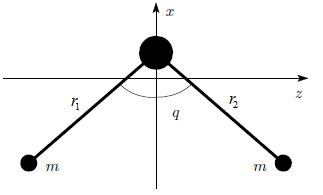
\includegraphics[width=0.4\textwidth]{../pictures/triatomic_full.png}
	\caption{Молекула $\ce{H2X}$ в подвижной системе отсчета.}
	\label{fig:triatomic_full}
\end{figure}

Выпишем координаты легких атомов в системе координат, связанной с центром масс.
\vverh
\begin{gather}
\left\{
\begin{aligned}
x_1 &= - r_1 \cos \lb \frac{q}{2} \rb \\
y_1 &= 0 \\
z_1 &= - r_1 \sin \lb \frac{q}{2} \rb 
\end{aligned}
\right. \quad \quad \quad
\left\{
\begin{aligned}
x_3 &= - r_2 \cos \lb \frac{q}{2} \rb \\
y_3 &= 0 \\
z_3 &= r_2 \sin \lb \frac{q}{2} \rb
\end{aligned}
\right.\notag
\end{gather}

Запишем кинетическую энергию в форме Лагранжа в подвижной системе координат. Используем формулы, приведенные в первой части, определяющие вид матриц $\bba$, $\bbA$, $\bbI$ в общем случае. Количество степеней свободы в данной модели равно $s = 3$, следовательно, размеры всех вышеперечисленных матриц будут равны $\dim \bba = \dim \bbA = \dim \bbI = 3 \times 3$. Путем несложных преобразований приходим к следующему виду матрицы тензора инерции (который в рамках данной модели не является диагональным):
\vverh
\begin{gather}
\bbI = \begin{pmatrix}
m \left( r_1^2 + r_2^2 \right) \sin^2 (\frac{q}{2}) & 0 & m \left( r_2^2 - r_1^2 \right) \sin (\frac{q}{2}) \cos(\frac{q}{2}) \\
0 & m (r_1^2 + r_2^2) & 0 \\
m \left( r_2^2 - r_1^2 \right) \sin(\frac{q}{2}) \cos(\frac{q}{2}) & 0 & m \left( r_1^2 + r_2^2 \right) \cos^2 (\frac{q}{2})
\end{pmatrix} \notag
\end{gather}

Составлять матрицы $\bba$, $\bbA$ будем таким образом, чтобы они давали правильные выражения кинетической энергии (в любом представлении) при использовании вектора обобщенных координат в форме $\begin{bmatrix} r_1 \\ r_2 \\ q \end{bmatrix}$. Матрица $\bba$ оказывается диагональной, причем пара диагональных элементов оказывается равной (в следствие идентичности, с точностью до номера, атомов $1$ и $3$): $a_{11} = a_{22} = m, \, a_{33} = \frac{m}{4} (r_1^2 + r_2^2)$. Матрица $\bbA$, в отличие от прошлой модели, не является нулевой, она содержит единственный ненулевой элемент: $A_{23} = \frac{m}{2} (r_2^2 - r_1^2)$. Заметим, что при фиксировании двух длин связи $r_2 = r_1 = r_0$, матрица $\bbA$ становится нулевой. \\
С учетом выполненных преобразований запишем кинетическую энергию лагранжевого вида в скалярной форме: 
\vverh
\begin{gather}
T_\mathcal{L} = \frac{1}{2} m \left(\dot{r}_1^2 + \dot{r}_2^2 + ( r_1^2 + r_2^2 ) \frac{\dot{q}^2}{4} \right) + \Omega_y m \frac{\dot{q}}{2} (r_2^2 - r_1^2 ) + \frac{1}{2} \vec{\Omega}^{\, \top} \, \bbI \, \vec{\Omega} \notag 
\end{gather}

Для перехода к кинетической энергии в форме Гамильтона применим формулы, полученные при помощи подхода Фробениуса к обращению блочных матриц. Достаточно длинные выкладки приводят к следующему виду элементов блочной матрицы $\bbG$, которая определяет вид кинетической энергии в гамильтоновой форме:
\vverh
\begin{gather}
\bbG_{11} = \ddfrac{r_1^2 + r_2^2}{2 m r_1^2 r_2^2}
\begin{bdmatrix}
\frac{1}{1 - \cos q} & 0 & \frac{r_1^2 - r_2^2}{r_1^2 + r_2^2}  \frac{1}{\sin q} \\
0 & 1 & 0 \\
\frac{r_{1}^{2} - r_{2}^{2}}{r_{1}^{2} + r_{2}^{2}} \frac{1}{\sin q} & 0 & \frac{1}{1 + \cos q}
\end{bdmatrix} \notag
\end{gather}

Матрица $\bbG_{12}$ содержит единственный ненулевой элемент $\left( \bbG_{12} \right)_{32} = - \ddfrac{r_2^2 - r_1^2}{2 m r_1^2 r_2^2}$. Матрица $\bbG_{11}$ является диагональной, причем так же как и матрица $\bba$, содержит пару одинаковых диагональных элементов. $\left( \bbG_{11} \right)_{11} = \left( \bbG_{11} \right)_{22} = \ddfrac{1}{m}$, $\left( \bbG_{11} \right)_{33} = \ddfrac{r_1^2 + r_2^2}{m r_1^{2} r_2^{\, 2}}$.
Приходим к следующей скалярной форме гамильтониана в гамильтоновом представлении:
\vverh
\begin{gather}
T_\mathcal{H} = \frac{1}{2} \left( \frac{J_x^2}{I_0 (1 - \cos(q))} + \frac{J_y^2}{2I_0} + \frac{J_z^2}{I_0 (1 + \cos(q))} + 2 \frac{r_1^2 - r_2^2}{r_1^2 + r_2^2} \frac{J_x J_z}{I_0 \sin(q)} \right) + \notag \\
+ \frac{r_1^2 - r_2^2}{2m r_1^2 \cdot r_2^2} J_y p + \frac{p_1^2}{2m} + \frac{p_2^2}{2m} + \frac{p^2}{I_0} , \notag
\end{gather}

\vlevo где было введено обозначение $I_0 = \ddfrac{2m r_1^2 r_2^2}{r_1^2 + r_2^2}$; $p$,$p_1$,$p_2$ -- обобщенные импульсы, сопряженные координатам $q$, $r_1$, $r_2$, соответственно.

Заметим, что при фиксировании координат $r_1 = r_2 = r_0$ ($p_1 = p_2 = 0$):
\vverh
\begin{gather}
I_0 = \frac{2m r_1^2 \cdot r_2^2}{r_1^2 + r_2^2} \quad \rightarrow \quad I_0 = m r_0^2, \notag 
\end{gather} 
и полученная кинетическая энергия для модельной системы с тремя степенями свободы переходит в кинетическую энергию для системы с одной деформационной степенью свободы.

Итак, приходим к слудующему виду модельного гамильтониана:
\begin{gather}
\mathcal{H} = \frac{1}{2} \left( \frac{J_x^2}{I_0 (1 - \cos q)} + \frac{J_y^2}{2 I_0} + \frac{J_z^2}{I_0 (1 + \cos q)} + 2 \frac{r_1^2 - r_2^2}{r_1^2 + r_2^2} \frac{J_x J_z}{I_0 \sin q} \right) + \frac{r_1^2 - r_2^2}{2m r_1^2 r_2^2} J_y p + \frac{p_1^2}{2m} + \frac{p_2^2}{2m} + \notag \\
+ \frac{p^2}{I_0} + U (r_1, r_2, q) \label{model_ham2}
\end{gather}

Потенциал $U(r_1, r_2, q)$ описывает потенциальную поверхность, зависящую от всех трех внутренних степенйе свободы. В первом приближении будем считать, что мы можем разбить потенциал на три независимых слагаемых, каждое из которое зависит от одной степени свободы: $U(r_1, r_2, q) = U_1 (r_1) + U_1 (r_2) + U (q)$. 
Руководствуясь теми же причинами, что были описаны в обсуждении первой модели, в качестве деформационного потенциала был выбран потенциал Пешля-Теллера. В качестве потенциала валетного типа использовался модельный потенциал гармонического осциллятора и реалистический потенциал Морзе. 
\vverh
\begin{gather}
\left[
\begin{aligned}
U(r_1, r_2, q) &= k (r_1 - r_0)^2 + k (r_2 - r_0)^2 + \frac{1}{2 I_0} \left( \ddfrac{V_{-}}{1 - \cos q} + \ddfrac{V_{+}}{1 + \cos q} \right) \\
U(r_1, r_2, q) &= D_e (1 - \exp (- a (r_1 - r_e))^2 + D_e (1 - \exp (- a (r_2 - r_e))^2 + \frac{1}{2 I_1} \left( \ddfrac{V_{-}}{1 - \cos q} + \ddfrac{V_{+}}{1 + \cos q} \right) 
\end{aligned}
\right. \notag
\end{gather}

(В рамках этой части переобозначим константу в потенциале Пешля-Теллера $I_1 = m r_0^2$.) \\
Константа жесткости $k$ гармонического осциллятора оценивалась по данным, приведенным в таблице \eqref{table1}. 
\vverh
\begin{gather}
\gamma = \frac{1}{\lambda} \quad \implies \quad 
\nu = \frac{c}{\lambda} = c \gamma \quad \implies \quad
\omega = 2 \pi \nu = 2 \pi c \gamma \quad \implies \quad
k = 4 \pi^2 c^2 \gamma^2 m , \notag 
\end{gather}
где $\gamma$ -- волновое число, а $\omega$ -- циклическая частота осциллятора.

\begin{figure}[H]
  \centering
	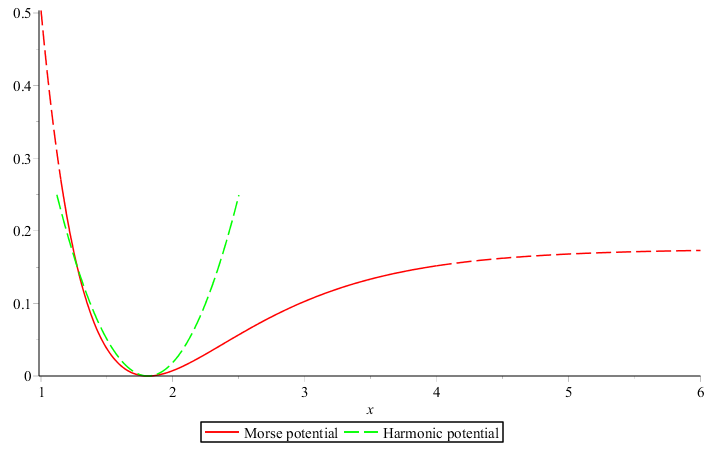
\includegraphics[width=0.75\textwidth]{../pictures/potentials.png}
	\caption{Графики гармонического потенциала и потенциала Морзе.}
\end{figure}


Для определения параметров потенциала Морзе была применена следующая процедура. Первая производная показывает, что потенциал Морзе достигает своего минимального значения при $r = r_e$. Аппроксимируя потенциал Морзе в окрестности точки минимума гармоническим потенциалом, выразим постоянную $a$. В качестве постоянной $D_e$ была взята энергия гидроксильной связи. 
\vverh
\begin{gather}
V(r) = D_e (1 - \exp (- a (r - r_e))^2 \notag \\
\frac{\mathrm{d}V}{\mathrm{d}r} = 2 a D_e \exp (- a (r - r_e)) (1 - \exp (-a (r - r_e))) 
\qquad \implies \qquad \frac{\mathrm{d}V}{\mathrm{d}r} \bigg{|}_{r_e} = 0 \notag \\
\frac{\mathrm{d}^2 V}{\mathrm{d}r^2} = 2 a^2 D_e \left[ 2 \exp (-a (r - r_e)) - 1 \right] \exp (-a (r - r_e)) \qquad \implies \qquad k = \frac{\mathrm{d}^2 V}{\mathrm{d}r^2} \bigg{|}_{r_e} = 2 a^2 D_e \notag \\
a = \sqrt{\ddfrac{k}{2D_e}} \notag
\end{gather}

Потенциал Морзе может быть проквантован аналитическим образом, его энергетический спектр имеет следующий вид:
\vverh
\begin{gather}
E_n = h \nu_0 \left( n + \frac{1}{2} \right) - \ddfrac{\left[ h \nu_0 \left( n + \frac{1}{2} \right) \right]^2 }{4 D_e}, \notag
\end{gather} 

\vlevo где $\nu_0 = \frac{a}{2 \pi} \sqrt{\ddfrac{2 D_e}{m}}$.